\documentclass[
a4paper,     %% defines the paper size: a4paper (default), a5paper, letterpaper, ...
% landscape,   %% sets the orientation to landscape
% twoside,     %% changes to a two-page-layout (alternatively: oneside)
% twocolumn,   %% changes to a two-column-layout
% headsepline, %% add a horizontal line below the column title
% footsepline, %% add a horizontal line above the page footer
% titlepage,   %% only the titlepage (using titlepage-environment) appears on the first page (alternatively: notitlepage)
% parskip,     %% insert an empty line between two paragraphs (alternatively: halfparskip, ...)
% leqno,       %% equation numbers left (instead of right)
% fleqn,       %% equation left-justified (instead of centered)
% tablecaptionabove, %% captions of tables are above the tables (alternatively: tablecaptionbelow)
% draft,       %% produce only a draft version (mark lines that need manual edition and don't show graphics)
10pt         %% set default font size to 10 point
% 11pt         %% set default font size to 11 point
% 12pt         %% set default font size to 12 point
]{scrartcl}  %% article, see KOMA documentation (scrguide.dvi)

\usepackage{graphicx}


%%%%%%%%%%%%%%%%%%%%%%%%%%%%%%%%%%%%%%%%%%%%%%%%%%%%%%%%%%%%%%%%%%%%%%%%%%%%%%%%
%%%
%%% packages
%%%
\usepackage[utf8]{inputenc}

%%% fontenc, ae, aecompl: coding of characters in PDF documents
\usepackage{dsfont}
\usepackage[T1]{fontenc}
\usepackage{ae,aecompl}

%%% amsmath, amssymb, amstext: support for mathematics
\usepackage{amsmath,amssymb,amstext}
\usepackage{bm}

%%% psfrag: replace PostScript fonts
\usepackage{psfrag}

\usepackage{xcolor}
\usepackage{subcaption}
\usepackage{placeins}
\usepackage{enumitem}
\usepackage{float}
\usepackage{wrapfig}

\usepackage{ifpdf}
\usepackage{amsfonts}
\newcommand{\RomanNumeralCaps}[1]
{\MakeUppercase{\romannumeral #1}}

\usepackage{todonotes}


%%%%%%%%%%%%%%%%%%%%%%%%%%%%%%%%%%%%%%%%%%%%%%%%%%%%%%%%%%%%%%%%%%%%%%%%%%%%%%%%
%%%
%%% define the titlepage
%%%

\subject{Exercise - Star/Galaxy Classification}   %% subject which appears above titlehead
\titlehead{Architecture of Machine Learning Systems} %% special heading for the titlepage

%%% title
\title{Report}

%%% author(s)
\author{Noah Ruhmer (11918092)}

%%% date
\date{\today{}}


%%%%%%%%%%%%%%%%%%%%%%%%%%%%%%%%%%%%%%%%%%%%%%%%%%%%%%%%%%%%%%%%%%%%%%%%%%%%%%%%
%%%
%%% begin document
%%%

\begin{document}

\pagenumbering{roman} %% small roman page numbers

%%% include the title
% \thispagestyle{empty}  %% no header/footer (only) on this page
 \maketitle

%%% start a new page and display the table of contents
% \newpage
%\tableofcontents

%%% start a new page and display the list of figures
% \newpage
% \listoffigures

%%% start a new page and display the list of tables
% \newpage
% \listoftables

%%% display the main document on a new page 
%\newpage

\pagenumbering{arabic} %% normal page numbers (include it, if roman was used above)

%%%%%%%%%%%%%%%%%%%%%%%%%%%%%%%%%%%%%%%%%%%%%%%%%%%%%%%%%%%%%%%%%%%%%%%%%%%%%%%%
%%%
%%% begin main document
%%% structure: \section \subsection \subsubsection \paragraph \subparagraph
%%%

\newpage
\section{Project Description}
This project aims to use data from the Sloan Digital Sky Survey (SDSS) to distinguish image patches as stars or galaxies.
The dataset provides image data spread all over the sky as seen from the earth, including coordinates of stars and galaxies.

An entire machine learning pipeline, from data collection up to model evaluation, is given in this project.
The report describes the steps of this pipeline and explains the reasons for selecting techniques and approaches.

The README.md file briefly describes the supplied code and how to locally execute the entire pipeline.
A docker container is also provided, which can be used to reproduce the results stated in this report more easily.

\section{Data Acquisition and Alignment}
For data acquisition, we first need to understand the data format provided by the SDSS and what data is stored.
We then download this data and realign images to have correctly aligned frames to work on.

\subsection{Data Format}
Data is recorded by the SDSS using an imaging camera that scans a strip of the sky.
A strip, also called run, consists of 6 parallel scanlines called camcol, each using a different filter for recording.
Each camcol is projected to a width of $2048$ pixels and between these camcols are small gaps that are covered in different overlapping runs.
A camcol strip is split into slightly overlapping smaller images of resolution $1489\times 2048$, which are called fields.

However, a camcol does consist of multiple spectral bands spanning the optical window.
These color channels are abbreviated \textbf{z, i, r, g, u} and cover the wavelength from infrared up to including ultraviolet.
These spectral bands are not recorded simultaneously but alternating, therefore not perfectly aligned.

The SDSS also provides coordinate data of stars and galaxies.
These are provided per camcol and are given as represented by a World Coordinate System (WCS).
This system uses spherical coordinates very similar to longitude and latitude to identify the direction of a strip in relation to the earth.

\subsection{Download}
The SDSS provides the data on their servers, and we can download frame data by specifying rerun, run, camcol, field and spectral band.
A rerun is simply reprocessing a run with different software and camera calibrations.
Coordinate data for stars and galaxies is provided per camcol.

\begin{figure}[h]
    \center
    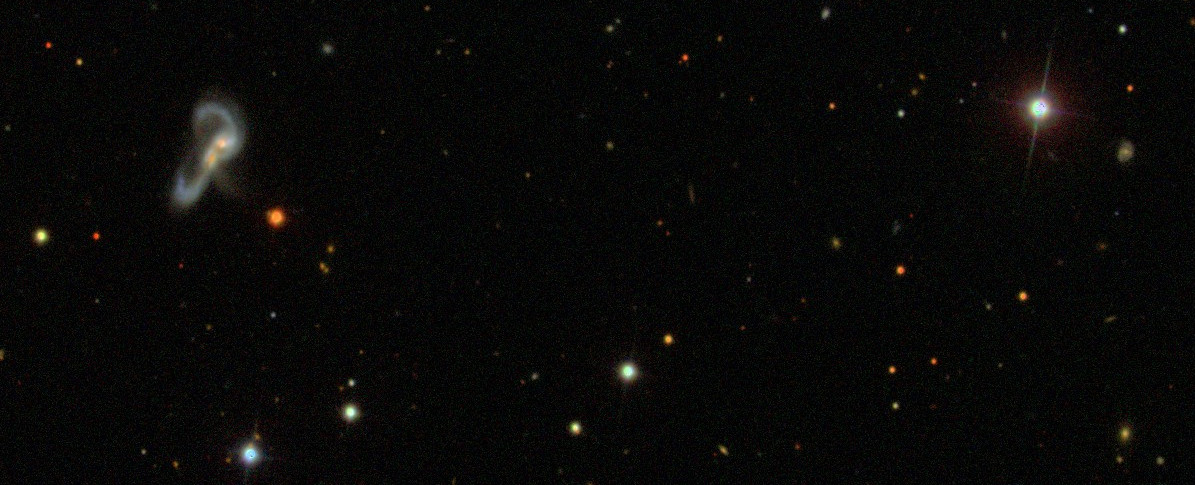
\includegraphics[width=\textwidth]{figures/crop_original}
    \caption{Raw RGB image after download}\label{fig:download_rgb}
\end{figure}
Visualized in Figure~\ref{fig:download_rgb} is a RGB cutout of an field after download.
Here we observe the image to be blurry and that near bright lights the red, green and blue streaks seem to be separated.
This visualizes the shift between the spectral bands and shows the need for alignment as next step in this pipeline.

\subsection{Alignment}
As the spectral bands for a field are not perfectly aligned, we must reproject the frames on top of each other to fix this mistake.
Each spectral band frame has a WCS, which can be used to realign all 5 frames to produce a single aligned 5-channel field.

The resulting aligned image would be of different sizes depending on the offset between spectral bands.
Unavailable channels of the resulting field are padded with $0$ to retain a constant field size.

\begin{figure}[h]
    \center
    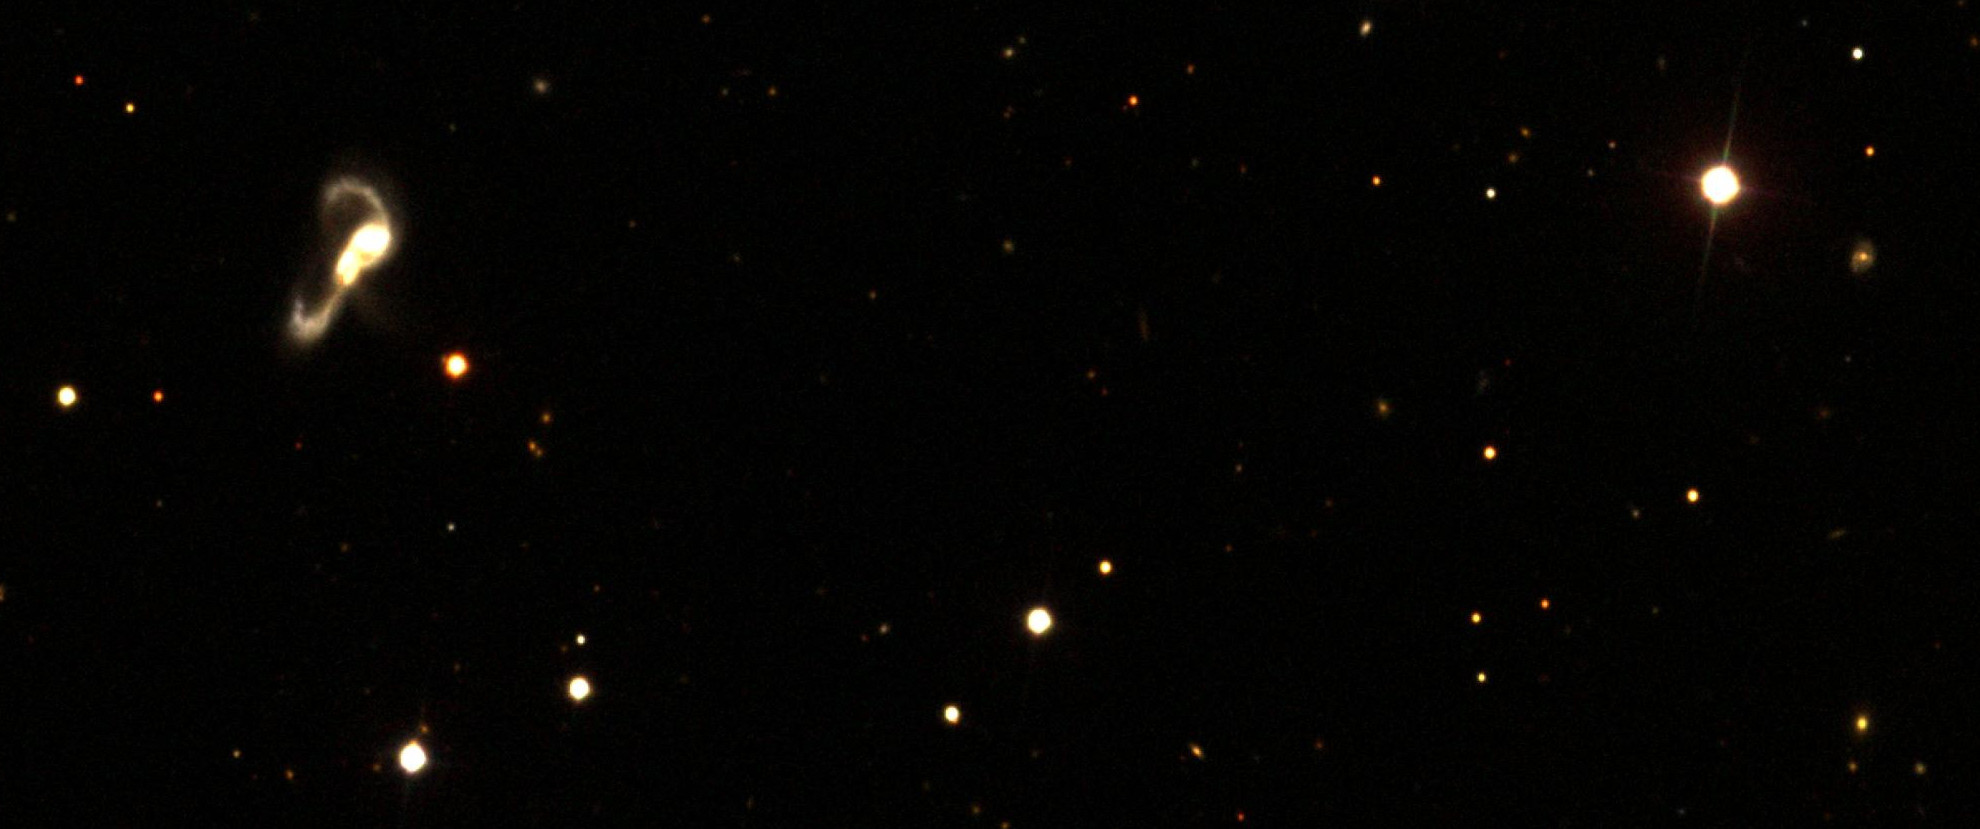
\includegraphics[width=\textwidth]{figures/crop_aligned}
    \caption{Aligned RGB image}\label{fig:aligned_rgb}
\end{figure}
Figure ~\ref{fig:aligned_rgb} shows the same cropout as in Figure~\ref{fig:download_rgb} but after the alignment step.
The previously blurry stars are now more sharp and distinct.
There are no color artifacts, yet smaller light sources are still hard to detect visually.

\subsection{Data statistics}
Aggregation over 10 fields of the data showed that the distribution of stars to galaxies is roughly $31.5\%$ to $68.5\%$.
This proportion can change for different fields but is usually relatively stable within a single run.
Over different runs this relation, or in general the amount of stars and galaxies within a field can also vary greatly.

Regarding the size of stars and galaxies the data has shown to be rather varying.
Visual inspection of different star coordinates show that some stars are merely a few or single pixel wide, while bigger galaxies although rare, may span more than 50 pixels.

The different spectral bands also usually coincide for stars and galaxies as long as data is extracted from the same camcol within a run.
Fields from other camcols have shifted color spectrum due to different filters being used in the camera system per camcol.

\section{Data Preparation}
We need to prepare our data for model training.
For this, we must consider the large size of a single field of $1489 \times 2048 \times 5 = 15247360$ float values.
This rather large data size is not practical and unnecessary for our star or galaxy classification task.
Instead, we can use smaller image patches that should contain sufficient information for the task and are more lightweight to train on.

We must also ensure a disjoint but similar training, validation and test data split.
This split is vital to train an unbiased model and correctly evaluate its performance.

\begin{figure}[h]
    \center
    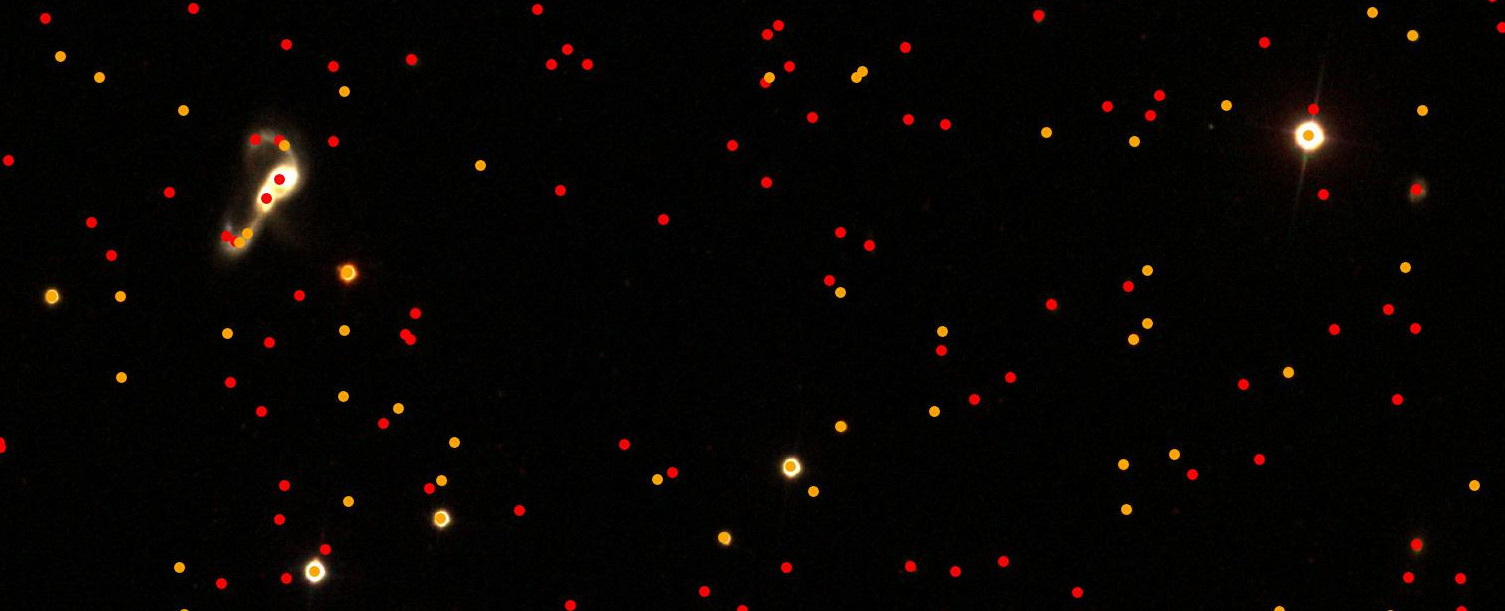
\includegraphics[width=\textwidth]{figures/crop_marked}
    \caption{Aligned RGB image}\label{fig:marked_rbg}
\end{figure}

The target coordinates for our stars and galaxies are visualized in Figure~\ref{fig:marked_rbg}.
We can compare this to Figure~\ref{fig:aligned_rgb} and see that some stars and galaxies are obvious for the human eye.
A problem is also that some galaxies and stars are very close too each other, and also that very bright light sources might overlap smaller ones.
These will be nearly impossible to predict based only on our image data.

\subsection{Patch Extraction}
The file containing the star and galaxy coordinates attributes a single coordinate to only a single field.
These WCS coordinates of stars and galaxies can be transformed into corresponding pixel coordinates.
We cut out a patch centered around the star or galaxy coordinate to extract these patches.
Experiments showed that a patch size of $25\times 25$ pixels is a promising tradeoff between runtime and model performance.

Shown in Figure~\ref{fig:patches} we can see two example patches showcasing not only different light intensity but also sizes of stars and galaxies.
These examples are not representative for the respective class, only showcasing 2 randomly chosen patches.
\begin{figure}[H]
    \centering
    \begin{subfigure}{.49\textwidth}
        \centering
        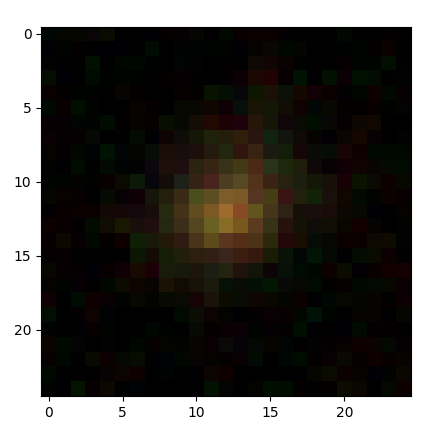
\includegraphics[width=\linewidth]{figures/star_patch}
        \caption{Star Patch}
    \end{subfigure}
    \begin{subfigure}{.49\textwidth}
        \centering
        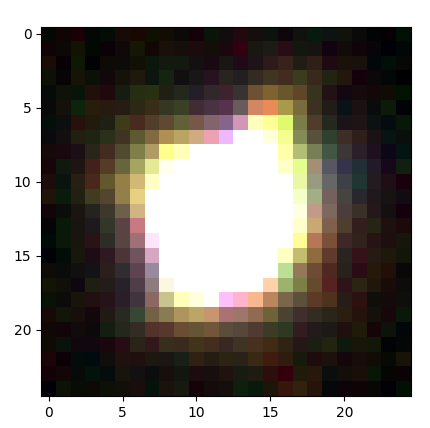
\includegraphics[width=\linewidth]{figures/gal_patch}
        \caption{Galaxy Patch}
    \end{subfigure}
    \caption{\label{fig:patches}Extracted $25 \times 25$ patches showcasing an example star and galaxy}
\end{figure}

\subsection{Training, Validation and Test Split}
We must carefully select data for the model to train on.
There cannot be any overlap between training, validation and test data which is challenging due to the overlapping fields.
Due to the nature of patch extraction, a patch might also contain pixels of stars or galaxies close to it.

We assign all stars and galaxies in a field to the same data bucket to ensure disjoint training, validation, and test sets.
This separation ensures that patches containing other data do not seep into the training, validation or test process and vice versa.
It is also important not to use adjacent fields as they overlap and could contain the same points multiple times but in different buckets.

As discussed in the previous chapter, the distribution of stars and galaxies within fields shifts greatly between runs and camcols.
To ensure similarity of the training, validation and test data distribution, only data from the same rerun, run and camcol is used.

\paragraph{Field Specification}
Only fields from rerun 301, run 8162 and camcol 6 have been used.
The fields were chosen randomly, under the condition that they cannot be adjacent.
The training uses a small (single frame) and a larger (7 frames) training set.
The same validation and test set are used for both training sets for comparable results.

\begin{itemize}
    \item Training-set small: 174
    \item Training-set large: 103, 111, 147, 174, 177, 214, 222
    \item Validation-set: 120, 228
    \item Test-set: 80
\end{itemize}


\section{Modeling and Tuning}
The task of our model is to perform binary classification between stars and galaxies.
We have a $5$ channel image patch as input and expect a single float value between $0$ and $1$  as output.
This value depicts the network's confidence to which class the image patch belongs.

To use backpropagation, we need a loss metric and therefore use the binary cross-entropy loss for this task.
Weight updates are performed using the Adam optimization algorithm.

\subsection{Model Selection}
The first experiment used a straightforward handcrafted convolutional neural network as a binary classifier.
It consists of 2 convolutional layers, a fully connected dense layer, and a single neuron activated by a sigmoid function as output.
This approach used no regularization techniques and performed surprisingly well without any tuning.

It was improved by adding dropout layers, $l_2$-normalization and avoiding over-fitting by early stopping on the validation loss.
Experiments with batch normalization, different amounts of layers, filters, nodes, kernel, and pooling sizes led to no significant performance improvement.
Adding the augmentation techniques listed above improved the model performance by a small margin.
The initial model seems, by luck, to perform exceptionally well, as many modifications led to no improvement.

By increasing the patch size, more complex architectures like a U-Net or a residual neural network (RNN) have been tried.
However, these architectures performed worse than the initial model and are not fit for the task due to the small input complexity when using patches.

A detailed description of the architectures of the base and improved model can be found in the appendix~\ref{subsec:model_arch}.

\pagebreak
\subsection{Model Tuning}
To optimize the improved model's stability and convergence, the networks parameters were fine-tuned manually.
Performed experiment results with different learning rates, dropout rates and regularization weights were compared and the best parameterizations were chosen for the final model.

Using early stopping on the validation loss after 5 epochs without improvement showed a good tradeoff of convergence and avoiding over-fitting on the training data.
A good tradeoff between runtime and performance was achieved by using 7 training frames, 2 validation frames and the reference test frame.

\begin{figure}[h]
    \begin{subfigure}{.5\textwidth}
        \centering
        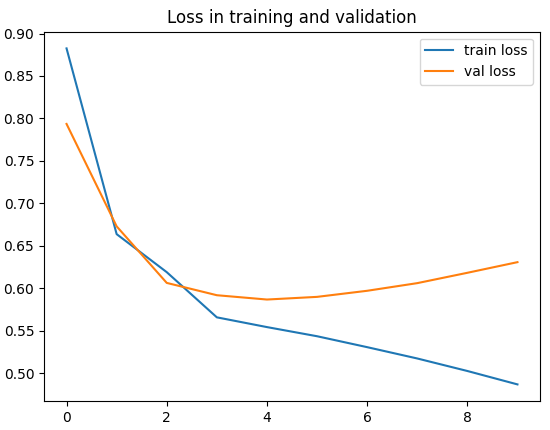
\includegraphics[width=\linewidth]{figures/base_model_loss}
        \caption{Base Model: Loss per epoch}
    \end{subfigure}
    \begin{subfigure}{.5\textwidth}
        \centering
        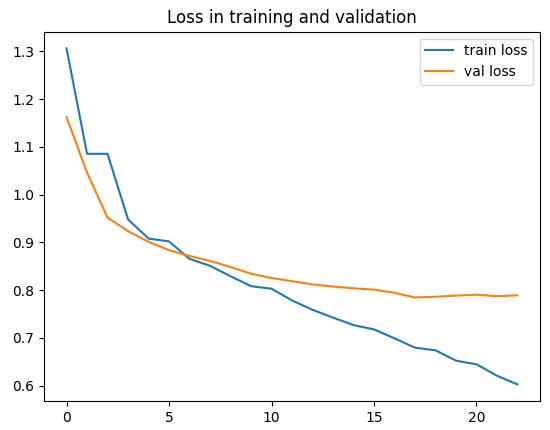
\includegraphics[width=\linewidth]{figures/reg_model_loss}
        \caption{Improved Model: Loss per epoch}
    \end{subfigure}
    \begin{subfigure}{.5\textwidth}
        \centering
        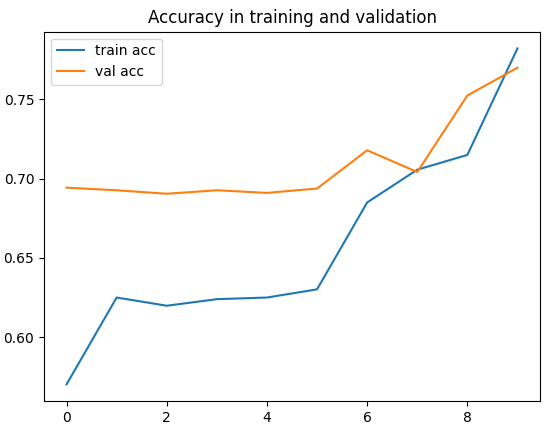
\includegraphics[width=\linewidth]{figures/base_model_accuracy}
        \caption{Base Model: Accuracy per epoch}
    \end{subfigure}
    \begin{subfigure}{.5\textwidth}
        \centering
        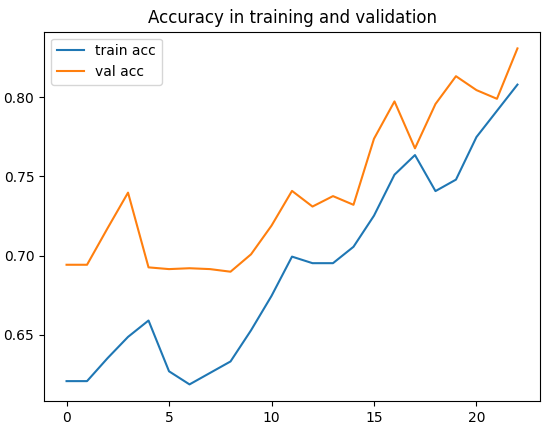
\includegraphics[width=\linewidth]{figures/reg_model_acc}
        \caption{Improved Model: Accuracy per epoch}
    \end{subfigure}
    \caption{\label{fig:model_comp}Model comparison based on training and validation loss and accuracy}
\end{figure}

As shown in Figure~\ref{fig:model_comp} we can see the loss and accuracy of both the base and regularized model using only a single frame as training data.
The base models loss converges pretty early and only achieves a validation accuracy around $75\%$.
Using the improved model with regularization techniques and fine-tuned hyperparameters trains for a longer time and before stopping and achieves a validation accuracy of around $82\%$.

The loss during training of the improved model is also higher due to the dropout layers which are only active during training.
This makes the training data more difficult to predict but is disabled for predicting on the validation data.

Overall, we can observe the fine-tuning and regularization of the convolutional neural network to be very effective.
Results on the same training set improve significantly and the runtime increase compared to the effect is negligible.

\subsection{Evaluation}
We want to evaluate the performance of the trained model.
As our task is binary classification, we can look at the confusion matrix of the predicted to actual labels.
A more direct metric would be to use accuracy, but the Matthews Correlation Coefficient (MCC) is better suited due to the imbalance in class distribution.
This report will state both metrics as the accuracy is more intuitive to read, but the MCC is more expressive in describing the full confusion matrix.

We should also compare the results to a baseline to get an intuition for the quality of the results.
In binary classification, randomly choosing the class gives already a $50\%$ accuracy.
Due to the imbalance in labels, a model always predicting the mode class would even achieve a $~74.6\%$ accuracy.

For both baselines the MCC is not meaningful as it is $0$ or not defined in the case of the mode-predictor.
This is only natural as there is no correlation between input and class label when picking at random.
When predicting the mode we have a constant output which cannot correlate with the input.

We expect our trained model to outperform the random and mode baseline.
These baselines are also a way of verifying that our model is working and something to relate our model performance to.

\begin{figure}[H]
    \centering
    \begin{subfigure}{.46\textwidth}
        \centering
        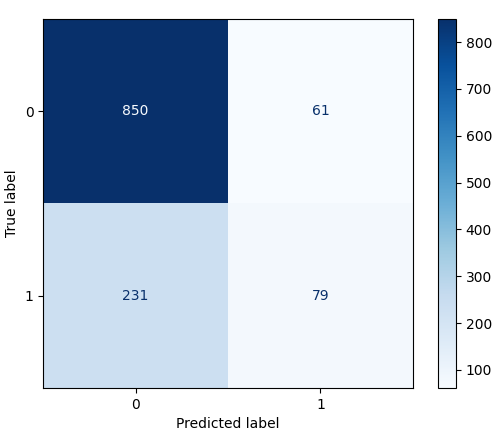
\includegraphics[width=\textwidth]{figures/basic_confusion}
        \caption{\label{fig:confusion_basic}Predictions of base model}
    \end{subfigure}
    \begin{subfigure}{.46\textwidth}
        \centering
        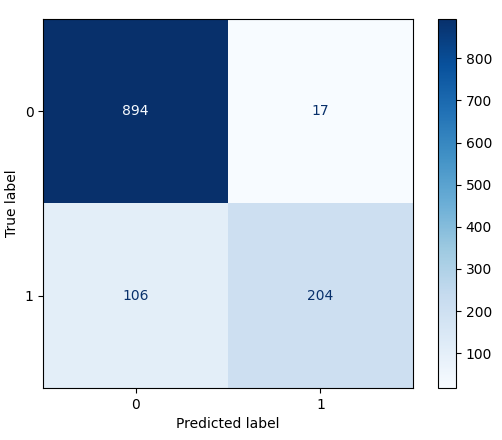
\includegraphics[width=\textwidth]{figures/improved_confusion}
        \caption{\label{fig:confusion_improved}Predictions of improved model}
    \end{subfigure}
    \caption{\label{fig:confusion_comp}Confusion Matrices of prediction on both models (labels: 0=galaxy, 1=star)}
\end{figure}

The prediction matrices of the first and the fine-tuned model are given in Figure~\ref{fig:confusion_comp}.
Data was collected by training the base model on the non-augmented single-frame training set and the improved model on the large training set.

Graph~\ref{fig:confusion_basic} shows that the basic model predicts something similar to the mode-baseline.
The model learned to mostly predict the galaxy class.
Therefore, the results are similar to the mode-baseline with an MCC of $0.257$ and an accuracy of $76.1\%$.

However, the improved model in Graph~\ref{fig:confusion_improved} was trained on the larger training set discriminate better between stars and galaxies.
It has increased the amount of correctly classified galaxies and stars.
The most errors are regarding stars (label 1).
These results are difficult to explain, but visual inspection seems to indicate that these errors mostly stem from different light sources overlapping the target.
Still, we the resulting model achieves an MCC of $0.723$ and an accuracy of $89.9\%$.

\section{Data Augmentation}
We can also use data augmentation to increase diversity in the training data artificially.
Although there is large amounts of data available, using data augmentation still increases the model performance and reduces the amount of data needed to download significantly.

Different image processing techniques can be combined to augment the data to be used in training.
These techniques should, however, transform the images in a way that still corresponds to the same class.
Thus, we must understand the data we work with and how it is generated.

Techniques like zooming, color shifting, shearing and artificial stars or galaxies have not been applied.
Color and size may be relevant characteristics to classify a star or galaxy.
And stars and galaxies are usually symmetric, which would be violated by shearing operations.

Lastly, one would first need to model how stars and galaxies look to generate artificial stars or galaxies.
This approach could work but highly depends upon the quality of generated stars and galaxies.
A simple generative model like a Gaussian Mixture Model (GMM) could be trained on the patch data and used to create new patches artificially.
Due to this project's scope, this approach has not been pursued further but could lead to promising results.

\subsection{Augmentations}
These augmentations are applied per extracted image patch and are only used for the model's training data.
We expect an increase in training loss but a decrease in validation loss, resulting in better model performance.

The following augmentations were tested and fine-tuned individually but can be applied combined to create an augmented training set.
A full augmentation of the training set with all possible combinations would increase the training data set size by a factor of $48$.
This significant increase of training data size leads to a higher diversity in the training set.

\paragraph{Rotation}
Rotating the images by $90, 180$ and $270$ degrees.

\paragraph{Reflection}
Reflecting the image diagonally and over one main axis.

\paragraph{Brightness Shift}
Shifting the intensity per channel by a normal distributed offset.

\paragraph{Blurring}
Applying a Gaussian Blur to the whole image patch.\\

Visualizations of these patch transformations are given in the appendix \ref{subsec:aug_trans}.

\subsection{Single Frame experiments}
Augmentations results on training-set small (25$\times$25):
  \begin{center}
    \begin{tabular}{||c c c c c c||}
     \hline
     Run & Augmentation & Train Loss & Train Accuracy & Val Loss & Val Accuracy \\ [0.5ex]
     \hline\hline
     1 & None               & 0.55745 & 0.79029 & 0.86818 & 0.82575 \\
     \hline
     2 & Rotation           & 0.46808 & 0.83161 & 1.06580 & 0.82247 \\
     \hline
     3 & Reflection         & 0.49307 & 0.82438 & 0.89858 & 0.85260 \\
     \hline
     4 & Brightness Shift   & 0.53758 & 0.80165 & 0.98318 & 0.81425 \\
     \hline
     5 & Blurring           & 0.57526 & 0.80579 & 1.01371 & 0.83123 \\
     \hline
     6 & Combination        & 0.35001 & 0.85541 & 0.91511 & 0.84986 \\
     \hline
    \end{tabular}
  \end{center}

\subsection{Multi Frame experiments}
Augmentations results on training-set large (25$\times$25):
  \begin{center}
    \begin{tabular}{||c c c c c c||}
     \hline
     Run & Augmentation & Train Loss & Train Accuracy & Val Loss & Val Accuracy \\ [0.5ex]
     \hline\hline
     1 & None               & 0.33072 & 0.87113 & 0.35818 & 0.85096 \\
     \hline
     2 & Rotation           & 0.30447 & 0.87712 & 0.28938 & 0.88219 \\
     \hline
     3 & Reflection         & 0.31343 & 0.87702 & 0.30119 & 0.89205 \\
     \hline
     4 & Brightness Shift   & 0.30958 & 0.87686 & 0.31151 & 0.89479 \\
     \hline
     5 & Blurring           & 0.31703 & 0.87558 & 0.30748 & 0.88384 \\
     \hline
     6 & Combination        & 0.30820 & 0.87786 & 0.27750 & 0.89096 \\
     \hline
    \end{tabular}
  \end{center}

\subsection{Augmentation Effects}
As illustrated in the 2 examples above, we can see that the impact of data augmentation is quite visible on both training sets.
We increase the models validation accuracy by $~2.5\%$ and $~4\%$ for the respective small and large training set.
Model performance trained on a singular augmented frame is comparable to training on 7 non-augmented frames.

The observed effect of combined augmentations is reduced in comparison to individual image augmentations.
It can be suspected that combining some augmentations creates similar kinds of diversity in the training data and reads to diminishing returns in regard to overall training data size.

\section{Conclusion}
This project provides a complete machine-learning pipeline to classify image patches from the SDSS as either star or galaxy.
The trained model has been evaluated on a test frame and achieves good prediction accuracy outperforming all set baselines.

With a simple convolutional neural network using small image patches as input, we achieve a good classification accuracy of $90.5\%$
and a matthew correlation score of $0.746$.
Both metrics significantly outperform our baselines and show that the classification of stars and galaxies trained on this model works and is meaningful.
We also can see that this classification task, although only binary is still not trivial.

Only using imaging data lets us distinguish stars pretty accurately from galaxies.
However it seems that stars are harder to classify than galaxies.
This might be explained due to usually relatively low brightness of stars compare to galaxies.

\subsection{Further Enhancements}
This project could be developed further by extending it to a multi-classification (sky, star, galaxy, both) task.
The same network could be used when using a softmax activation as output and the cross-entropy loss to optimize for.
Training data would need to be extended to contain sky patches and ensure that the class imbalance in the training data does not take overhand.
In this case, the extracted patches should not overlap too much.

An analysis of the model could also be performed using explainable AI techniques.
This could confirm the expectations that the convolutional network is more influenced by the center of extracted patches.

The model could also be extended by including a light sources inferred distance to earth in the model input.
Because the current model uses only image data, which does not contain information about the distance and therefore size of an object.

Data augmentation could be further improved by using a trained generative model to generate artificial training data.
Depending on the generative model, this could also help to extract more relevant features of stars and galaxies which could be more focused in the model, or highlighted using data augmenation.


\subsection{Problems}
Current image alignment and patch extraction use $0$ padding to retain the original frame size.

It should also be noted that the current preprocessing is not fit to work with adjacent fields due to the duplication of stars and galaxies.
This could be overcome by cropping the fields down to non-overlapping sizes.

Due to a limited amount of computational resources and time this project did only use a limited amount of training data.
A improved performance of the classifier is to be expected by increasing the size of the training set and adapting the model accordingly.
\pagebreak
\section{Appendix}
\label{sec:appendix}

\subsection{Model Architectures}
\label{subsec:model_arch}
Description of the convolutional neural network built with TensorFlow:
\begin{verbatim}
Model: "base_model"
___________________________________________________________________
 Layer (type)                      Output Shape            Param #
===================================================================
 conv2d (Conv2D)                   (None, 23, 23, 32)         1472
 max_pooling2d (MaxPooling2D)      (None, 11, 11, 32)            0
 conv2d_1 (Conv2D)                 (None, 9, 9, 64)          18496
 max_pooling2d_1 (MaxPooling2D)    (None, 4, 4, 64)              0
 flatten (Flatten)                 (None, 1024)                  0
 dense (Dense)                     (None, 128)              131200
 dense_1 (Dense)                   (None, 1)                   129
===================================================================
Total params: 151,297
Trainable params: 151,297
Non-trainable params: 0
___________________________________________________________________


Model: "regularized_model"
___________________________________________________________________
 Layer (type)                      Output Shape            Param #
===================================================================
 conv2d_2 (Conv2D)                 (None, 23, 23, 32)         1472
 max_pooling2d_2 (MaxPooling2D)    (None, 11, 11, 32)            0
 spatial_dropout2d (SpatialDropout2D)   (None, 11, 11, 32)       0
 dropout (Dropout)                 (None, 11, 11, 32)            0
 conv2d_3 (Conv2D)                 (None, 9, 9, 64)          18496
 max_pooling2d_3 (MaxPooling2D)    (None, 4, 4, 64)              0
 spatial_dropout2d_1 (SpatialDropout2D)  (None, 4, 4, 64)        0
 dropout_1 (Dropout)               (None, 4, 4, 64)              0
 flatten_1 (Flatten)               (None, 1024)                  0
 dense_2 (Dense)                   (None, 128)              131200
 dropout_2 (Dropout)               (None, 128)                   0
 dense_3 (Dense)                   (None, 1)                   129
===================================================================
Total params: 151,297
Trainable params: 151,297
Non-trainable params: 0
___________________________________________________________________
\end{verbatim}

\subsection{Image Transformations}
\label{subsec:aug_trans}

The Figures~\ref{fig:aug1},\ref{fig:aug2},\ref{fig:aug3},\ref{fig:aug4},\ref{fig:aug5} show the transformation of the image patches.
For simplicity of observations the visualization is in grayscale and of a single spectral band.
Still, all augmentations are applied over all spectral bands of each image patch.
\begin{figure}[h]
    \center
    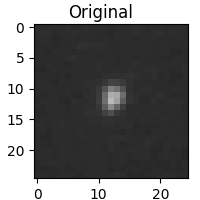
\includegraphics[width=0.3\textwidth]{figures/augment_original}
    \caption{Original Patch}\label{fig:aug1}
\end{figure}
\begin{figure}[h]
    \center
    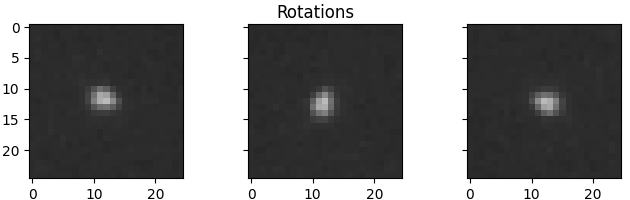
\includegraphics[width=0.95\textwidth]{figures/augment_rotations}
    \caption{Patch in 3 augmented rotations}\label{fig:aug2}
\end{figure}
\begin{figure}[h]
    \center
    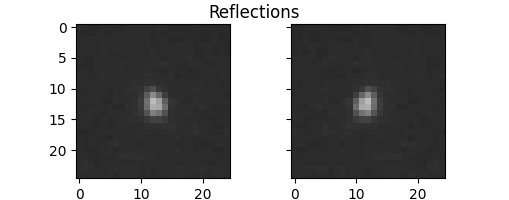
\includegraphics[width=0.75\textwidth]{figures/augment_reflections}
    \caption{Patch in 2 augmented reflections}\label{fig:aug3}
\end{figure}
\begin{figure}[h]
    \center
    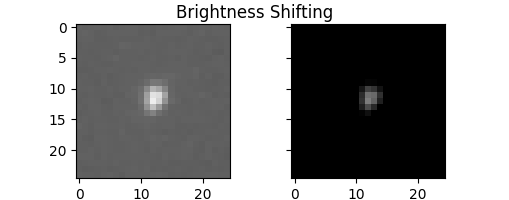
\includegraphics[width=0.75\textwidth]{figures/augment_shift}
    \caption{Patch with 2 different brightness shift augmenations}\label{fig:aug4}
\end{figure}
\begin{figure}[h]
    \center
    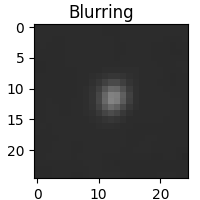
\includegraphics[width=0.3\textwidth]{figures/augment_blur}
    \caption{Patch with a gaussian blur applied}\label{fig:aug5}
\end{figure}



%%%
%%% end main document
%%%
%%%%%%%%%%%%%%%%%%%%%%%%%%%%%%%%%%%%%%%%%%%%%%%%%%%%%%%%%%%%%%%%%%%%%%%%%%%%%%%%
\end{document}